\chapter{Obsługa programu}
Uruchamiamy program
\begin{figure}[H]
	\centering
	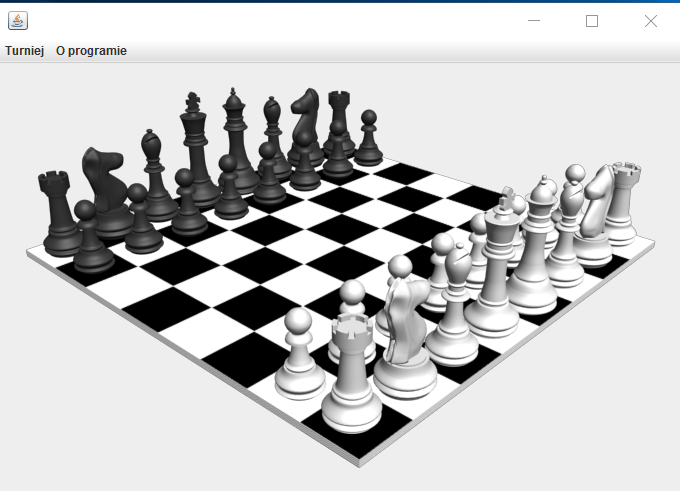
\includegraphics[width=10cm]{fig/1}
	\caption{Główne okno programu}
	\label {fig:glowne_okno_programu} 
\end{figure}
Z menu "Turniej" możemy wybrać opcję lub użyć skrótu klawiaturowego
\begin{figure}[H]
	\centering
	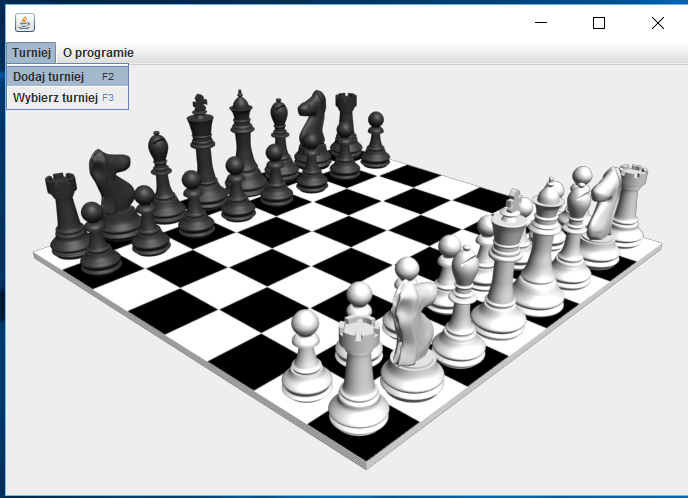
\includegraphics[width=10cm]{fig/2}
	\caption{Wybór turnieju}
	\label {fig:wybor_turnieju} 
\end{figure}
Jeżeli wybierzemy opcję "Dodaj turniej" musimy nadać mu nazwę
\begin{figure}[H]
	\centering
	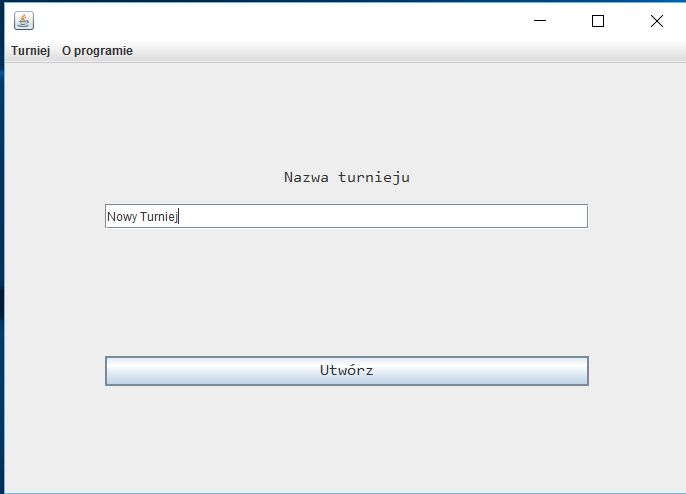
\includegraphics[width=10cm]{fig/3}
	\caption{Wybór nazwy turnieju}
	\label {fig:wybor_nazwy_turnieju} 
\end{figure}
Uczestnika turnieju możemy dodać na 2 sposoby:
\begin{enumerate}
	\item losowo
	\item uzupełniając jego dane
\end{enumerate}
\begin{figure}[H]
	\centering
	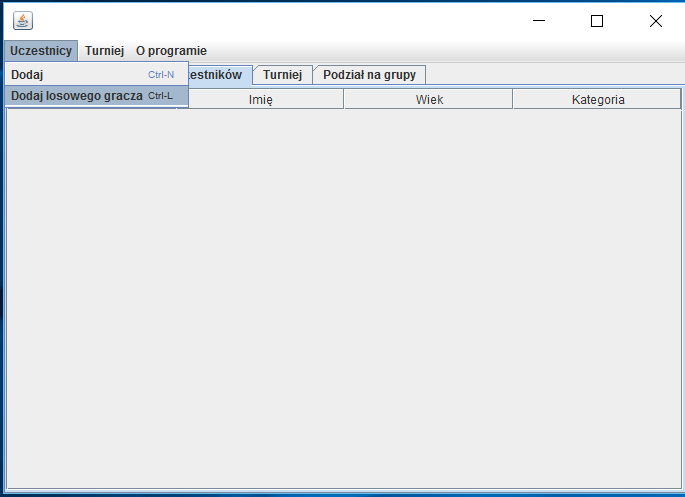
\includegraphics[width=10cm]{fig/4}
	\caption{Dodawanie uczestnika do turnieju}
	\label {fig:dodawanie_uczestnika_do_turnieju} 
\end{figure}
Wpisujemy dane użytkownika, kategorie możemy wybrać z listy
\begin{figure}[H]
	\centering
	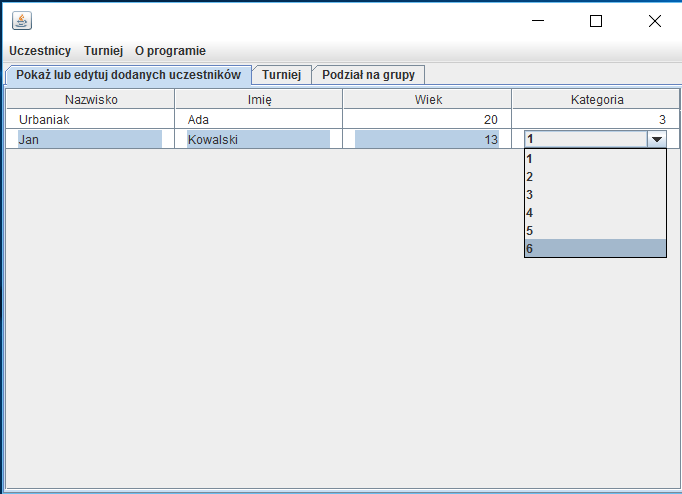
\includegraphics[width=10cm]{fig/5}
	\caption{Wybór kategorii}
	\label {fig:wybor_kategorii} 
\end{figure}
Istnieje możliwość usunięcia zawodnika z listy.\\
Klikamy PPM na wierszu w którym znajdują się dane zawodnika którego chcemy usunąć i wybieramy opcję "usuń" 
\begin{figure}[H]
	\centering
	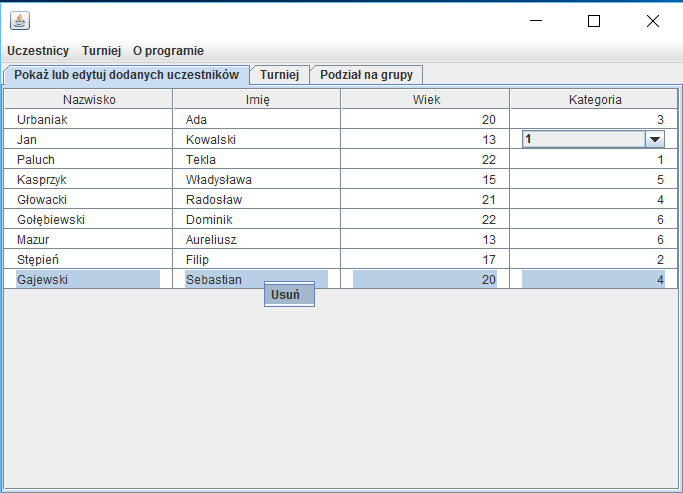
\includegraphics[width=10cm]{fig/6}
	\caption{Usuwanie zawodnika z listy}
	\label {fig:Usuwanie_zawodnika_z_listy} 
\end{figure}
W zakładce turniej możemy ustawic parametry turnieju takie jak:
\begin{enumerate}
	\item nazwa turnieju
	\item rok
	\item czas trwania pojedyńczej rozgrywki - minimum 1 minuta, maksimum 20 minut
	\item ilość drużyn - program wskaże optymalną ilość grup, którą można zmienić
	\item ilość szachownic - minimum 2, maksimum 20 
\end{enumerate}
Po ustawieniu żądanych parametrów program wyświetli:
\begin{itemize}
	\item liczbę rozgrywek
	\item przewidywany czas trwania eliminacji
\end{itemize}



\begin{figure}[H]
	\centering
	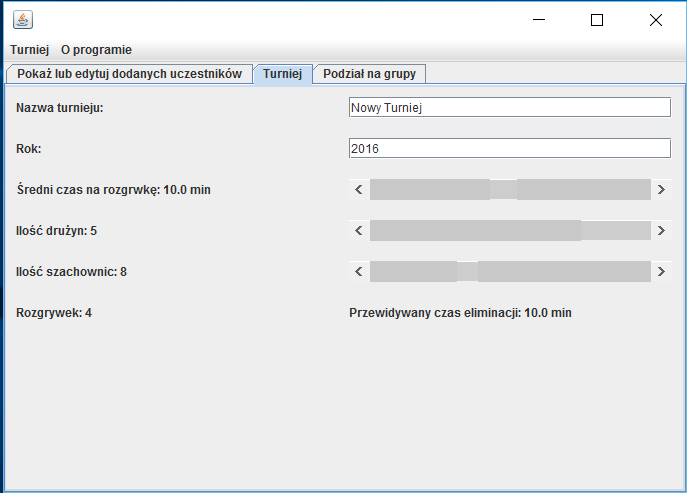
\includegraphics[width=10cm]{fig/7}
	\caption{Zakładka turniej}
	\label {fig:zakladka_turniej} 
\end{figure}
W zakładce "Podział na grupy" z menu "Sortowanie graczy" możemy wybrać sposób sortowania uczestników według kryteriów widocznych poniżej
\begin{figure}[H]
	\centering
	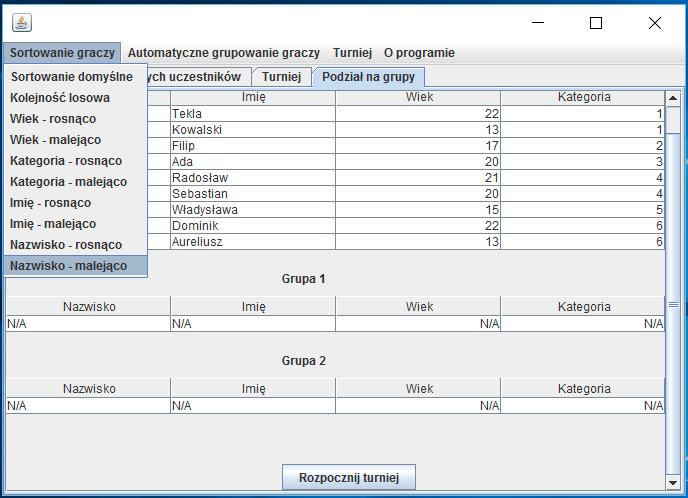
\includegraphics[width=10cm]{fig/8}
	\caption{Sposoby sortowania uczestników}
	\label {fig:Sposoby_sortowania_uczestnikow} 
\end{figure}
Zawodników możemy przydzielić do grup automatycznie
\begin{figure}[H]
	\centering
	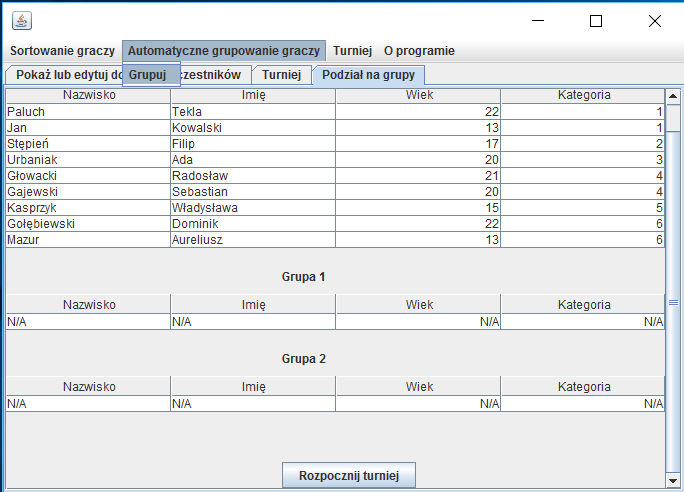
\includegraphics[width=10cm]{fig/9}
	\caption{Automatyczny przydział do grup}
	\label {fig:Automatyczny_przydzial_do_grup} 
\end{figure}
Zawodnika do grupy możemy przydzielić ręcznie klikając PPM i wybierając z listy grupę do której chcemy przydzielić uczestika
\begin{figure}[H]
	\centering
	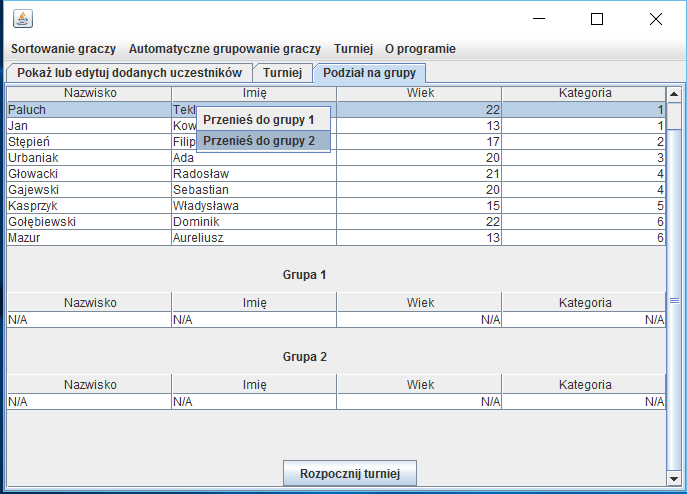
\includegraphics[width=10cm]{fig/10}
	\caption{Reczny przydział do grup}
	\label {fig:Reczny_przydzial_do_grup} 
\end{figure}
Jeżeli przydzielimy wszystkich zawodników do grup możemy rozpocząć turniej
\begin{figure}[H]
	\centering
	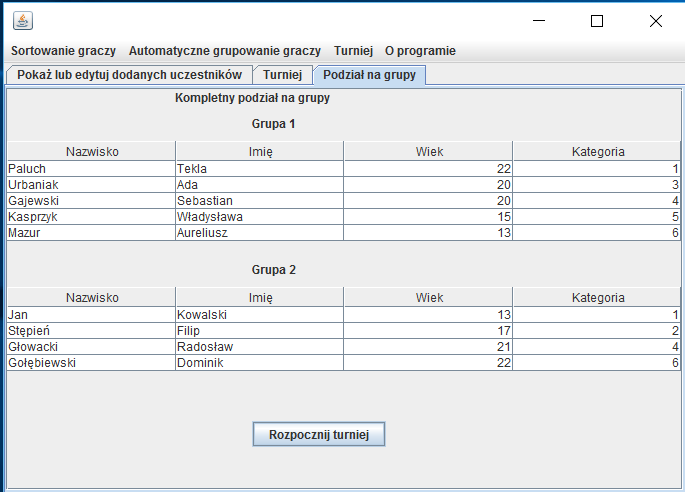
\includegraphics[width=10cm]{fig/11}
	\caption{Rozpoczęcie turnieju}
	\label {fig:rozpoczecie_turnieju} 
\end{figure}
Rozgrywki które mogą się odbyć zostają podświetlone na zielono\\
Zwycięzcę rozgrywki możemy wybrać z listy lub za pomocą skrótu klawiaturowego:
\begin{itemize}
	\item "b" - wygrywa kolor biały
	\item "c" - wygrywa kolor czarny
	\item "r" - remis
\end{itemize}

\begin{figure}[H]
	\centering
	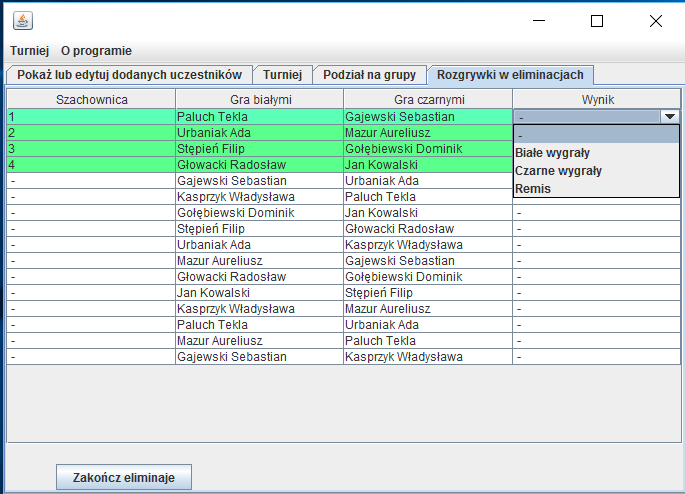
\includegraphics[width=10cm]{fig/12}
	\caption{Możliwe rozgrywki}
	\label {fig:mozliwe_rozgrywki} 
\end{figure}

\begin{figure}[H]
	\centering
	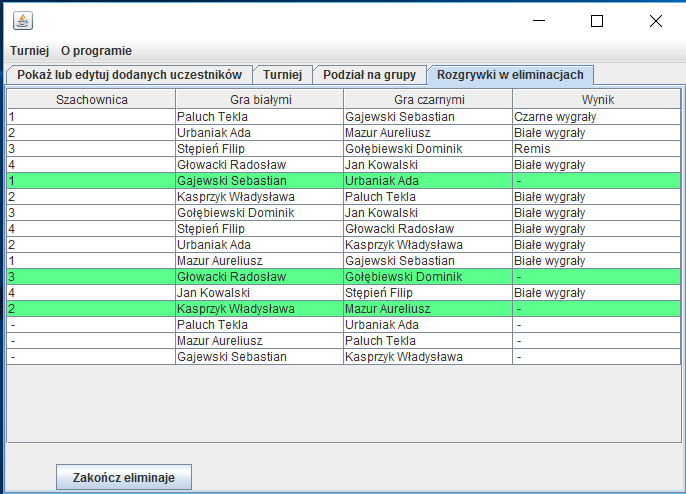
\includegraphics[width=10cm]{fig/13}
	\caption{Możliwe rozgrywki}
	\label {fig:mozliwe_rozgrywki_2} 
\end{figure}
Po ustaleniu wyników wszystkich rozgrywek możemy zakończyć eliminacje
\begin{figure}[H]
	\centering
	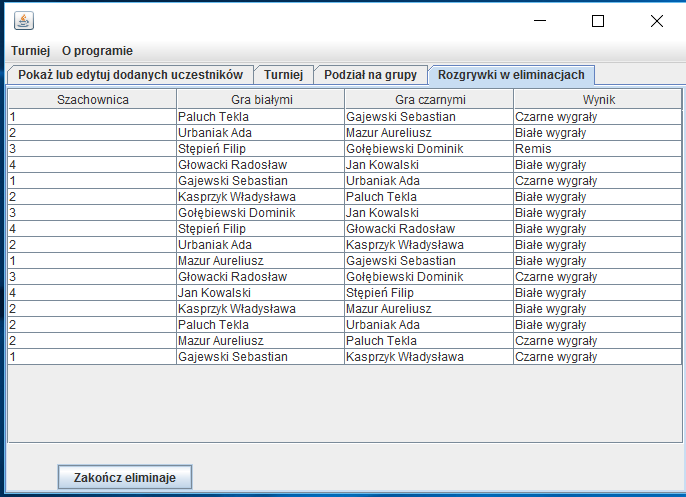
\includegraphics[width=10cm]{fig/14}
	\caption{Wybór zawodników do finału}
	\label {fig:wybor_zawodnikow_do_finalu} 
\end{figure}
Przechodzimy do zakładki "Wybór graczy do finałów"\\
Z każdej grupy musimy wybrać co najmniej jednego zawodnika który będzie brał udział w finale
\begin{figure}[H]
	\centering
	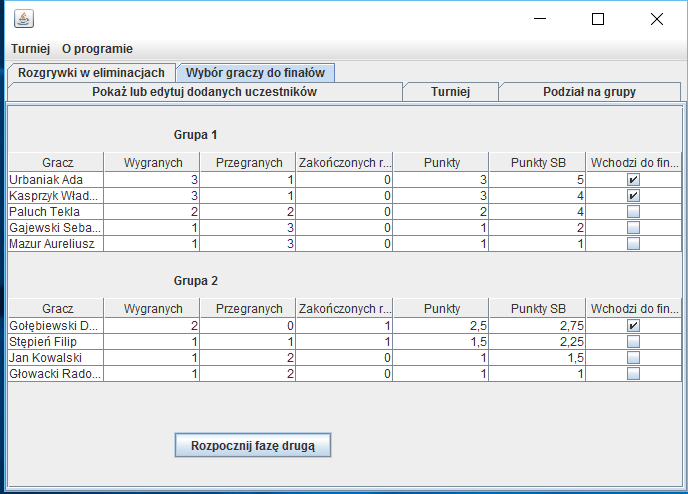
\includegraphics[width=10cm]{fig/15}
	\caption{Wybór graczy do finału}
	\label {fig:rozgrywka_finalowa_1} 
\end{figure}
Jeżeli zawodnicy którzy dostali się do finału grali ze sobą wcześniej, nie grają ponownie. Przyjęty zostaje wynik z poprzedniej rundy.
\begin{figure}[H]
	\centering
	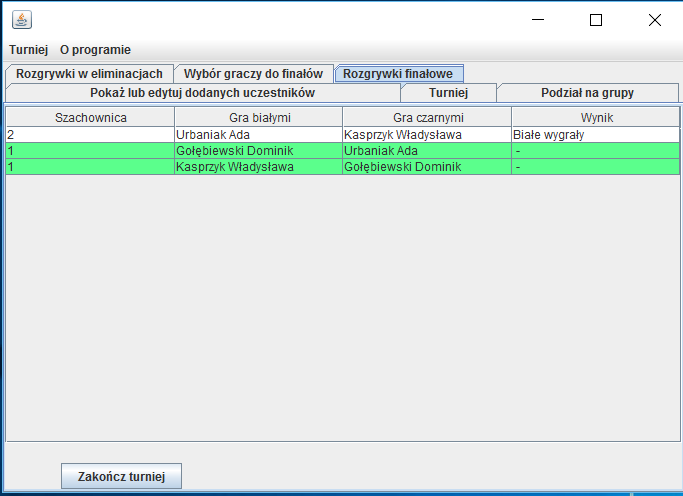
\includegraphics[width=10cm]{fig/16}
	\caption{Rozgrywki finałowe}
	\label {fig:rozgrywka_finalowa_2} 
\end{figure}

W zakładce "Wyniki turnieju" wyświetlone zostają wyniki z podziałem na miejsca
\begin{figure}[H]
	\centering
	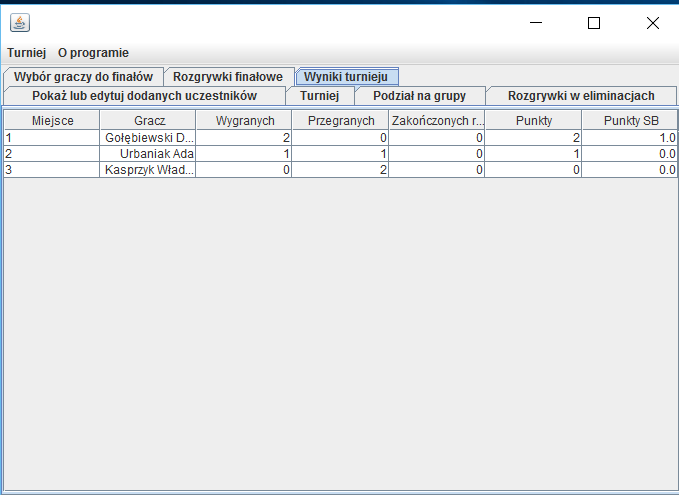
\includegraphics[width=10cm]{fig/17}
	\caption{Wyniki turnieju}
	\label {fig:wyniki_turnieju} 
\end{figure}
Po rozpoczęciu turnieju w zakładce "Pokaż lub edytuj dodanych uczestników" po kliknięciu PPM na wiersz z danymi uczestnika możemy wybrać opcję "Dyskwalifikuj". 
\begin{figure}[H]
	\centering
	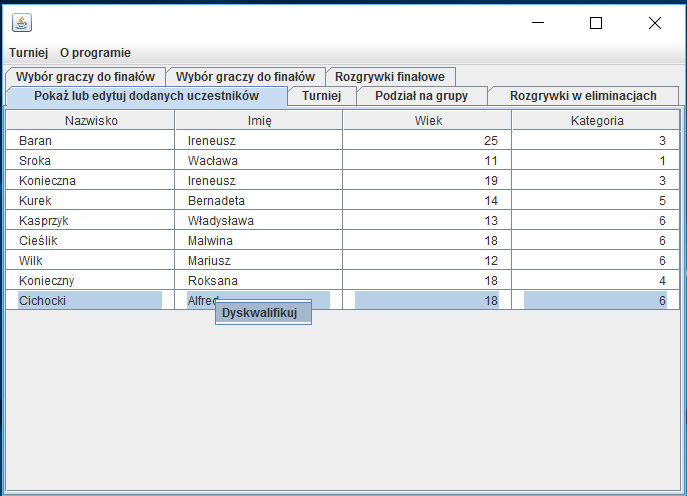
\includegraphics[width=10cm]{fig/18}
	\caption{Dyskwalifikacja zawodnika}
	\label {fig:dyskwalifikacja} 
\end{figure}
\textbf{Uwaga!!!} Z opcji dyskwalifikacji należy korzystać bardzo ostrożnie, tej operacji \textbf{nie} można cofnąć.
\begin{figure}[H]
	\centering
	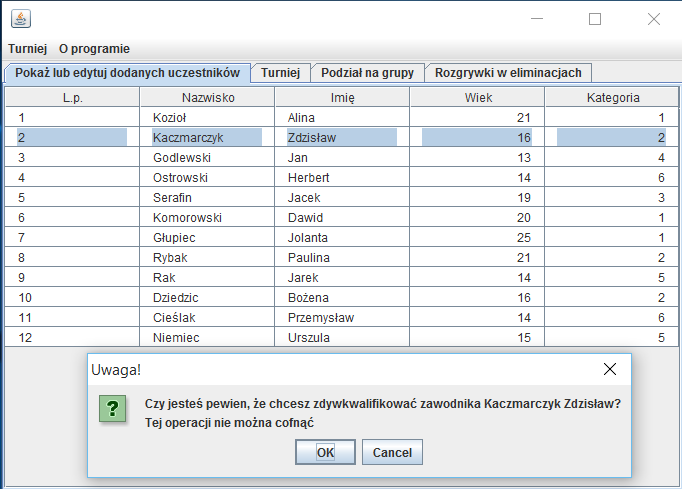
\includegraphics[width=10cm]{fig/19}
	\caption{Potwierdzenie dyskwalifikacji}
	\label {fig:dyskwalifikacja_potwierdzenie} 
\end{figure}
Jeżeli zawodnik rozegrał już jakieś pojedynki to nie zostają one anulowane a kolejne w których miał brać udział przegrywa walkowerem (przeciwnik dostaje 1 punkt), do nazwiska zawodnika zostaje dodane oznaczenie dyskwalifikacji "*d"
\begin{figure}[H]
	\centering
	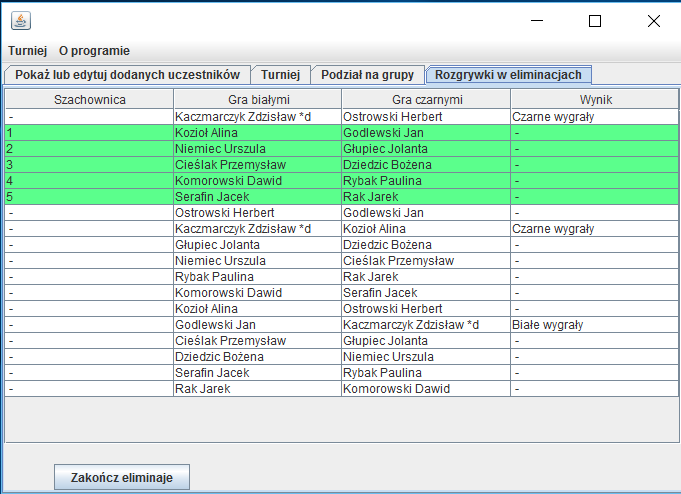
\includegraphics[width=10cm]{fig/20}
	\caption{Tabela wyników po dyskwalifikacji uczestnika}
	\label {fig:dyskwalifikacja_tabela} 
\end{figure}